% -*- japanese-LaTeX -*-
% 
% 
% Copyright (c) 2006-2014, Hiroyuki Ohsaki.
% All rights reserved.
% 
% $Id: paper.tex,v 1.4 2020/08/27 16:31:02 ohsaki Exp ohsaki $
% 
%% \documentclass[12pt,a4paper,titlepage,dvipdfmx]{jarticle}
\documentclass[12pt,a4paper,titlepage,dvipdfmx]{article}
\usepackage{insertfig}
\usepackage{palatino}
\usepackage{setspace}
\usepackage{url}

\usepackage{tabularx}
\usepackage{cite}
\usepackage{amsmath}
\usepackage{amssymb}
\usepackage{caption}
\usepackage{algorithmic}
\usepackage{algorithm}
\usepackage{insertfig}
\usepackage{times}
\usepackage{txfonts}
\usepackage{url}
\usepackage{enumerate}

\usepackage{revhistory}
%% \importrevisions
%\renewcommand{\baselinestretch}{1.0}

\renewcommand{\algorithmicrequire}{\textbf{Input:}}
\renewcommand{\algorithmicensure}{\textbf{Output:}}

\newcommand{\insertsubfig}[3][0]{ \subfigure[#3]{
    \label{fig:#2}
    \includegraphics[width=#1\columnwidth]{./../figure/b4_graduation_report/#2.eps}}}

\newcommand{\Gc}{\widehat{G}}
\newcommand{\Vc}{\widehat{V}}
\newcommand{\Ec}{\widehat{E}}
\newcommand{\xv}{\mathbf{x}}
\newcommand{\yv}{\mathbf{y}}

\newcommand{\Gest}{\tilde{G}}


\title{\LARGE \bf A Study on Efficient Link Fidelity\\ Measurement in Quantum Networks}


\author{\Large Shun Yamachika}

\date{\Large March 2026 \\[10mm]
  School of Engineering \\
  Kwansei Gakuin University
}

\doublespace

\begin{document}

\maketitle

\section*{ABSTRACT}
量子ネットワークにおいて、量子鍵配送（QKD）や分散量子計算（DQC）などのアプリケーションを高品質に実行するためには、通信リンクの忠実度（Fidelity）を正確かつ効率的に評価することが不可欠である。量子リンクの品質評価手法として確立されているNetwork Benchmarking（NB）は、状態準備および測定（SPAM）誤差の影響を分離して平均忠実度を推定できるロバスト性を有する。しかし、NBでは量子ビットの往復回数（バウンス数）が増えるにつれて信号強度が減衰し、それに伴い測定データの統計的な分散も変動する「不均一分散性（Heteroscedasticity）」が生じる。そのため、従来の解析で一般的に用いられる最小二乗法（OLS）の等分散性の仮定は成立せず、限られた測定リソースから得られる情報を最大限に活用できていないという課題があった。

本研究では、NBにおける推定精度を向上させるため、観測データの分散構造に基づき動的に重み付けを行う重み付き最小二乗法（Weighted Least Squares: WLS）を導入した評価手法を提案する。NetSquidを用いた数値シミュレーションにより、異なるリンク品質および測定リソース下での推定精度を評価した結果、WLSはOLSと比較して推定値の標準誤差を有意に低減できることが示された。特に高忠実度領域（$\alpha=0.99$）においては約80\%の改善が確認され、提案手法の有効性が実証された。本手法は、追加のハードウェアリソースを要することなく、データ処理アルゴリズムの改善のみで量子ネットワークの忠実度評価精度を向上させるものである。


\section*{Keywords}
Quantum network, Network Benchmarking (NB), Link fidelity estimation, SPAM robustness, Weighted Least Squares (WLS), Heteroscedasticity
\newpage

\tableofcontents
\newpage

\listoffigures
\newpage

\listoftables
\newpage


\section{Introduction}
\label{sec:intro}
量子コンピュータ間を接続する量子ネットワークは、次世代の通信基盤として大きな期待が寄せられている。量子ネットワークは、量子ビット（qubits）を用いて量子システム間で情報を伝送する技術であり、量子鍵配送（Quantum Key Distribution: QKD）、分散量子計算（Distributed Quantum Computing: DQC）、および量子センシングといった、古典的なインターネットでは実現不可能なアプリケーションを可能にするためである\cite{wehner2018quantum}。

量子ネットワーク上で高信頼な通信を実現するには、高い忠実度（Fidelity）を持つ量子通信リンクを選択し利用することが不可欠である。量子情報は本質的に脆弱であり、光ファイバー等の物理リンクにおける伝送損失や、環境ノイズ、およびゲート操作の不完全性によって、量子状態の劣化(デコヒーレンス)が容易に引き起こされる\cite{nielsen2010quantum}。また、量子複製不可能定理（No-Cloning Theorem）により、古典信号のように量子状態を複製して増幅することができないため、通信品質の維持は極めて困難である\cite{wootters1982single}。量子ネットワークのアプリケーションのパフォーマンスは、量子通信リンクの品質、すなわち忠実度に依存しているため量子ネットワークにおいて高品質なアプリケーションを実現するためには、高い忠実度を持つリンクを選択し、利用することが重要である。

したがって、信頼性の高い通信を実現するためには、ネットワーク内のリンク品質（特にエンタングルメントリンクの忠実度）を正確かつ効率的に評価・監視するプロセスが求められる。また、量子リンクの忠実度は環境条件の変化や機器の経時劣化によって変動するため、一度の評価ではなく継続的な監視が必要となる。

近年、量子ネットワークリンクの品質評価手法として、HelsenとWehnerによって提案されたNB(Network Benchmarking)が採用されるようになった\cite{helsen2023benchmarking}。本手法が広く採用される主たる理由は、評価に用いる量子状態の作成や読み出しを行うデバイス自体のエラー（State Preparation And Measurement: SPAMエラー）の影響を受けずに、通信路の品質のみを正確に抽出できるロバスト性にある。

NBの基本原理は、量子計算機の評価におけるゴールドスタンダードとされるRB(ランダム化ベンチマーク)の手法を通信路に応用したものである\cite{magesan2012characterizing, emerson2005scalable}。具体的には、リンク間で量子ビットを複数回往復（バウンス）させつつ、ランダムな操作によってノイズの性質を平均化（チャネル・トワリング）するプロセスをとる。これにより、物理的なノイズの複雑な詳細を簡略化し、信号強度が往復回数 $m$ に応じて単純に減衰していく挙動を作り出すことができる 。この減衰過程を指数関数モデル$\bar{b}_m = A p^{2m}$に当てはめることで、定数項 $A$ に吸収されるデバイス固有のSPAM誤差と、脱分極パラメータ $p$ および忠実度を推定する。ここで$\bar{b}_m$はバウンス数 $m$ における平均生存確率である。

NBは高精度なリンク評価を可能にする一方で、その測定コストは無視できない課題となっている。NBプロトコルでは、SPAMエラーを除去するために多数のバウンス（往復）と、統計的有意性を確保するための多数のショット（測定の繰り返し）が必要となる。測定に必要な量子もつれ（エンタングルメント）は生成コストが高いため、実運用中のネットワークにおいて全リンクに対して頻繁にNBを実行することは現実的ではない。

測定コストの削減に向けて、近年ではサンプリング戦略の効率化に関する研究が進められている\cite{liu2024linkselfie, wang2025learning, li2025fortuna}。しかし、集めたデータのフィッティング手法については、従来手法と同じ最小二乗法を踏襲しており、より効率的に情報量を抽出する余地がある。現行のNBにおけるフィティングでは、一般的に最小二乗法（Ordinary Least Squares: OLS）が用いられており\cite{helsen2023benchmarking}、すべてのバウンス回数 $m$ ごとの生存確率が統計的に同等の分散を持つ（等分散性）と仮定している。実際には、バウンス回数 $m$ が増加して信号が減衰するにつれ、観測される生存確率の分散構造は変動するため、各データ点の信頼性は均一ではない。特に、総測定コストを抑えるためにバウンス回数 $m$ の範囲を限定する場合、この分散の不均一性（不均一分散性）が推定精度に与える影響はより顕著となる。不均一な分散を持つデータに対して最小二乗法を適用することは、統計的に最適ではなく、推定された忠実度の不確実性を増大させる要因となる。

また、NBの基本原理となったRBでも特定のシーケンスを繰り返す実験では、シーケンスごとのエラー発生率のばらつきにより、シーケンス長によって生存確率の分散が異なることからWLSによるフィッティングが検討されてきた。RBにおけるゲートシーケンスの適用 (長さ $m$)はNBの状態の往復バウンス (回数 $m$)に相当するものである。Multiqubit randomized benchmarking using few samples\cite{helsen2019multiqubit}ではOLSの代替として反復再重み付き最小二乗法（IRLS）の使用を強く推奨しており、反復再重み付き最小二乗法を用いることで、データの分散構造を正しく反映したフィッティングが可能となり、結果として、従来考えられていたよりもはるかに少ないサンプル数（シーケンス数）で厳密な信頼区間を得ることができると証明した。Sampling Strategy Optimization for Randomized Benchmarking\cite{itoko2021sampling}では論文中で「実務においては通常の最小二乗法（OLS）よりも、重み付き最小二乗法（WLS）推定量を用いることが、よりタイトな推定を提供すると仮定されている」と述べており、重み付き最小二乗法の使用を標準的なアプローチとして扱っている。

量子ネットワークリンクの低い忠実度とそれに伴う生存確率の急激な減衰は、RB以上に統計的分散の変動を大きくするため、データの信頼性に応じた重み付け（WLS）を検討するべきである。RBで扱う量子ゲートの忠実度は通常非常に高く（99.9\%以上）、RBにおける生存確率は数百、数千のゲートシーケンスを経ても緩やかにしか減衰しない。対して、量子ネットワークリンク（特に長距離光ファイバーや、不完全なスワッピング操作を含むリンク）の忠実度は量子ゲートに比べて低い場合が多い。リンク間で量子ビットを $m$ 回往復させるバウンスや量子ゲートで特定のシーケンス(長さ $m$)を適用することは、数理的にはリンクの実効的な忠実度 $f$ を $m$ 回乗算すること（$f^m$）と等価である。よって、基底となる $f$ の値が低いNBにおいては、この累乗効果により生存確率がRBに比べて急速に消失することとなる。この急激な減衰過程において、分散の不均一性はRB以上に顕著になると考えられる。したがって、従来のRBで許容されていた等分散性を仮定する単純な最小二乗法（OLS）よりも、データの信頼性に応じた重み付けを行う手法（WLS等）の必要性がRB以上に高まると考えられる。

本研究では、限られた量子リソース下での推定不確実性を最小化することを目的とし、測定ごとに変動し得るノイズ特性へ柔軟に適応するため、取得したデータから分散構造を動的に推定する「適応的分散モデルベースWLS (Adaptive Variance-Model-based WLS)」を提案する。

本手法により、追加の測定リソースを消費することなく、推定される忠実度の相対不確実性を低減させることが可能となる。これは、量子ネットワークの運用効率を向上させ、より高品質な量子通信サービスの提供に寄与するものである。

本手法は以下の2つのステップで構成される。

\begin{itemize}
    \item \textbf{分散傾向の動的推定 (On-the-fly Variance Estimation):} 通常のOLSによる暫定的なフィッティングを行い、その残差から実験環境固有の分散関数（シーケンス長 $m$ と分散の相関関係）を導出する。
    \item \textbf{重み付き推定の適用 (Weighted Estimation):} 導出された分散関数の逆数を統計的重みとして採用し、WLSによる再フィッティングを行うことで、より信頼性の高いパラメータ推定を実現する。
\end{itemize}



\newpage


\section{Related Works}
\label{sec:relatedworks}
量子ネットワークリンクの品質評価手法は、ネットワークのアーキテクチャや発展段階、評価目的に応じて多様なアプローチが提案されてきた。これらの手法は大きく「エンタングルメントの検証」「直接伝送チャネルの推定」「ネットワーク全体の機能認証」の3つに分類でき、それぞれが固有の特徴と適用範囲を有している。本章では、これらの関連研究を概観した上で、本研究が依拠するNetwork Benchmarking（NB）の位置づけを明らかにする。

量子リピータネットワークに代表されるエンタングルメントベースのネットワークでは、生成・配布された量子もつれの品質評価がリンク品質の評価に直結する。エンタングルメントを厳密に特徴付ける手法として、ベル不等式の破れを検証するベル試験と、観測統計のみから共有状態を認証するセルフテスティングが挙げられる。ベル試験では、2つのノードが特定の基底で測定を行い、その相関がCHSH不等式などの古典的限界を超えるか否かを確認することで、リンクが量子的性質を保持していることを証明する\cite{clauser1969proposed}。セルフテスティングは、測定デバイスの内部構造を信頼せずに（Device-Independent）、ベル不等式の破れの大きさなどから共有状態が目標のエンタングルメント状態にどれだけ近いかを認証する手法であり\cite{mayers2004self}、量子鍵配送（QKD）のセキュリティ証明において重要な役割を果たしている。量子状態トモグラフィ（QST）は、生成されたエンタングルメント状態の密度行列を完全に再構成する手法であり、状態に関する完全な情報を提供する\cite{james2001measurement}。QSTでは、状態を複数の異なる測定基底（パウリ基底の組み合わせなど）で観測し、その統計から元の状態を推定する。測定回数は量子ビット数nに対して指数関数的に増大するため、主に少数量子ビット系の詳細な状態解析に用いられる\cite{haffner2005scalable}。この測定コストの増大という課題に対しては、線形回帰を用いた適応的な推定手法などが検討されており、より少ない測定回数で効率的に状態を再構成する試みが行われている\cite{qi2017adaptive, mu2020quantum}。

また、完全な状態再構成を行わずに特定の特性のみを抽出するアプローチも重要である。初期の研究としては、少数のパウリ測定から直接忠実度を推定するDirect Fidelity Estimation\cite{flammia2011direct}が知られている。近年、この概念を拡張したClassical Shadows（古典的シャドウ）を用いた効率的な状態検証手法が発展している。Hsin-Yuan Huangらが提案した「Shadow Overlap」プロトコル\cite{huang2020predicting}は、ランダムパウリ測定を用いたわずかな単一量子ビット測定で、ターゲット純粋状態$|\psi\rangle$と実験で生成された状態$\rho$との忠実度$\langle\psi|\rho|\psi\rangle$を推定するものである。

直接伝送ベースのリンクや、リンクを抽象的な量子チャネルとしてモデル化する場合には、チャネル特性を評価する手法が用いられる。量子プロセス・トモグラフィ（QPT）は、リンクを量子チャネル$\Lambda$として捉え、その入出力関係を完全に記述する手法である\cite{chuang1997prescription}。QPTにより、チャネルがどのような種類のエラー（脱分極、位相緩和、振幅減衰など）を引き起こすかを詳細に診断することが可能となる。Classical Shadowsをプロセス評価に応用した「ShadowQPT」は、チャネルのChoi行列を確率的に再構成する手法であり、完全なQPTと比較して対数的なサンプル数でチャネル特性を推定できる\cite{levy2024classical}。本手法は、チャネルの詳細なエラー構造を効率的に把握する必要がある場合に有用である。より理論的な側面では、リンクの究極的な性能限界である量子容量（Quantum Capacity）を推定する研究が進められている。量子チャネルの容量計算は超加法性のため一般に困難であるが、「Flagged Extensions（フラグ付き拡張）」と呼ばれる手法により、チャネル容量の厳密な上界を導出することが可能となった\cite{kianvash2022bounding}。これらの理論的成果は、ネットワーク設計段階における性能限界の把握に貢献している。また、こうした物理層の複雑性や不完全性を隠蔽し、信頼性の高い通信サービスとして上位レイヤに提供するためのリンク層プロトコルの設計も進められている\cite{dahlberg2019link}。

物理的なリンク単体の評価にとどまらず、ネットワーク全体の価値や構造を測る指標も提唱されている。「量子ネットワークユーティリティ（UQN）」は、ネットワークがユーザーにもたらす総体的な価値を定量化するフレームワークであり、QKD、分散量子計算、センシングなど様々なアプリケーションの効用関数の総和として定義される。UQN\cite{vardoyan2024quantum}における効用はレート（速度）と忠実度の関数であり、ネットワークリソースの最適配分（QNUM: Quantum Network Utility Maximization）の理論的基盤を提供している。量子ネットワーク科学（QNS）は、複雑ネットワーク科学を量子ネットワークに応用した新興分野である\cite{biamonte2019complex}。QNSでは、ネットワークのトポロジー構造（グラフ理論的性質）とエンタングルメント性能（忠実度、生成確率）を結びつけ、忠実度で重み付けされた「量子中心性」や、特定の忠実度閾値を超えたリンクのみで構成される有効トポロジーの解析などが行われている\cite{cuquet2009entanglement}。これらの研究は、物理的接続と量子的接続性の乖離を体系的に理解する枠組みを提供している。

以上の関連研究に対し、NBは量子メモリネットワーク段階以上のシステムにおいて、伝送チャネルの平均忠実度をSPAMエラーの影響を受けずに推定する手法として提案されたものである\cite{helsen2023benchmarking}。NBは、RB（ランダム化ベンチマーク）の一般化された理論的枠組み\cite{helsen2022general}やその統計的性質に関する解析\cite{harper2019statistical}を背景とし、リンク間で量子ビットを往復させながらランダム操作によってノイズを平均化するプロセスを通じて、単一の品質指標である平均忠実度を抽出する。

\subsection{Recent Advances in Efficient NB Protocols}
この限られた測定リソース（サンプル数）の中で、いかに効率よく高忠実度のリンクを特定するかという課題に対し、近年、強化学習の一種である多腕バンディット問題（Multi-Armed Bandit: MAB）の枠組みを応用した研究が2024年から2025年にかけて相次いで提案されている\cite{liu2024linkselfie, wang2025learning, li2025fortuna}。ここでの課題は、未知の忠実度を持つ多数のリンクの中から、最小限の試行回数で最も高品質なリンクを特定することである。NBをサブルーチンとして組み込んだMABベースのアルゴリズムが提案され、従来の手法と比較して劇的な効率化を達成している。

これらの研究は、NBが単なる静的な測定ツールから、動的なネットワーク制御アルゴリズムの中に組み込まれるアクティブなセンシング機能へと進化していることを示している。NBが広く採用される理由は、SPAMエラーを分離できる堅牢性、スケーラブルな品質推定、および物理層の抽象化という3つの特性にある。第一に、不確実な環境下での自律的な意思決定において、NBはその堅牢性から主要な学習アルゴリズムの基盤として採用されている。ネットワークトポロジやノードのパラメータが未知である状況では、測定器のエラーを排除できるかどうかが学習の収束を左右する。BeQuP\cite{wang2025learning}やFortuna\cite{li2025fortuna}といった最新のルーティング研究では、NBがSPAMエラーを分離できる点に着目し、バンディットアルゴリズムにおける信頼できるフィードバック機構として組み込んでいる。第二に、詳細な物理情報へのアクセスが制限される大規模ネットワークにおいて、NBはスケーラブルな品質推定手法として機能する。NBのマルチノードプロトコルは、古典ネットワークにおけるpingコマンドの量子版（Quantum Ping）として、中継ノードの詳細な情報を隠蔽したままエンドツーエンドのパス品質を計測できる\cite{helsen2023benchmarking}。この特性は、QBGP\cite{liu2024quantum}やLinkSelFiE\cite{liu2024linkselfie}におけるトポロジ非依存な経路選択の理論的基盤となっている。第三に、物理層の複雑性を抽象化し、上位レイヤが扱いやすい形式で情報を提供する点においても、NBの有用性は際立っている。完全なトモグラフィが提供する高次元データとは異なり、NBはリンク品質を単一のスカラー値に要約する。この特性により、Minerva\cite{li2024minerva}のようなアプリケーション層でのQoS制御など、量子物理の複雑さを隠蔽した古典的な最適化アプローチが可能となっている。これらはサンプリングの効率化には成功しているが、事後処理であるフィッティング精度の向上については議論されていない。
\newpage



\section{概要}
\label{sec:概要}
本研究では、量子ネットワークにおけるリンク品質を効率的に評価するための
手法として、Helsen と Wehner によって提案されたネットワークベンチマー
キング（Network Benchmarking, NB）を基盤とし、その推定精度を向上させる
改良手法を提案する。NBは量子計算機の特性評価において広く用いられるラン
ダム化ベンチマーキング（Randomized Benchmarking, RB）を量子ネットワー
クに適用したものであり、量子ネットワークリンクを特徴づける量子チャネル
の平均忠実度を推定することができる。本手法は実装が容易であり、状態準備
および測定（State Preparation and Measurement, SPAM）誤差に対する頑健
性を備えている。

本章では、まずNBの理論的枠組みを紹介し、続いて我々が導入した重み付き最
小二乗法による改良について述べる。


\subsection{ネットワークモデル}
\label{sec:ネットワークモデル}

NBを適用する量子ネットワークは、複数のノードとそれらを結ぶ接続から構成
される抽象的なモデルとして記述される。各ノードは大文字（A, B, ...）で
表記し、ノード間の接続は方向を持つ矢印（A $\to$ B）で表現する。これら
のノードと接続は、物理的なネットワーク構成要素を抽象化したものである。

量子ネットワークの発展段階に関する Wehner らの分類に従えば、NBが対象と
するノードは以下の3つの機能を有することが求められる。

第一に、量子状態をメモリに保持する能力である。これは各ノード A に対し
てメモリレジスタ $\mathcal{H}_A$ を割り当てることでモデル化される。こ
のレジスタは特定の初期状態 $\rho_A$ に初期化可能であり、測定演算子の集
合（POVM）$\{E_A^{(i)}\}_{i \in I}$ によって読み出すことができる。典型
的な例として、初期状態には全零状態 $|0\rangle$ を、測定には計算基底測
定を用いることが挙げられる。

第二に、保持された量子状態に対して量子演算を実行する能力である。これは
ゲート集合 $\mathbb{G}$ から選択された量子ゲート $U$ の適用としてモデル
化される。理想的にはこのゲート集合は普遍的、すなわち任意のユニタリ演算
がゲート集合の元の組み合わせによって実現可能であることが望ましいが、NB
の実行にはより弱い条件で十分である（詳細は後述する）。

第三に、ノード A からノード B へ量子状態を伝送する能力である。この機能
は、もつれを用いたテレポーテーションなど様々な物理的手段で実装され得る
が、ここでは抽象的な機能として扱う。NBが主として評価の対象とするのは、
この量子状態伝送の品質である。


\subsection{ノイズと平均忠実度}
\label{sec:ノイズと平均忠実度}
量子デバイスにおけるノイズは、一般に量子チャネルによってモデル化される。
量子チャネルは行列を行列に写す線形写像（超作用素）であり、量子状態を量
子状態に写すという物理的な妥当性を保証する性質を持つ。以下では量子チャ
ネルを $\Lambda$ で表記し、状態 $\rho$ に対するチャネルの作用を
$\Lambda(\rho)$ と記す。

本研究では、各ノードおよび接続に関連するノイズを以下のように量子チャネ
ルで表現する。ノード A における状態準備に伴うノイズを $\Lambda_A^{SP}$、
測定に伴うノイズを $\Lambda_A^M$ で表す。また、ノード A で実行される量
子演算 $U$（超作用素として $U(\rho) = U\rho U^\dagger$ と表記）に付随す
るノイズを $\Lambda_A^U$ で表す。これは、ノード A が状態 $\rho$ にゲー
ト $U$ を適用するよう指示された場合、実際の出力が $(\Lambda_A^U U)(\rho)
= \Lambda_A^U(U\rho U^\dagger)$ となることを意味する。さらに、ノード A
からノード B への量子伝送リンク A $\to$ B に対しては、伝送過程で生じる
ノイズを表す量子チャネル $\Lambda_{A \to B}$ を割り当てる。一般に
$\Lambda_{A \to B} \neq \Lambda_{B \to A}$ であるが、両者が等しくなる
特殊な場合も存在する。

ネットワークリンク A $\to$ B を量子チャネルとしてモデル化することで、
このリンクの品質を定量的に評価することが可能となる。リンクの品質評価は、
本質的には量子チャネル $\Lambda_{A \to B}$ が恒等チャネル（理想的な無
ノイズ伝送）をどの程度良く近似しているかを問うことに帰着する。この近似
の度合いを定量化する最も一般的な指標の一つが、量子チャネル $\Lambda$
の平均忠実度 $F(\Lambda)$ である。これは以下のように定義される：
\begin{equation}
F(\Lambda) = \int d\psi \, \mathrm{Tr}[\Lambda(|\psi\rangle\langle\psi|)|\psi\rangle\langle\psi|]
\end{equation}
ここで積分はすべての純粋状態 $|\psi\rangle$ について一様に行われる。こ
の量は、チャネル $\Lambda$ の作用によって一般的な量子状態がどの程度変
化するかを測定するものと解釈でき、チャネルの平均的な振る舞いを捉えてい
る。平均忠実度は量子計算機における演算品質を報告する際の標準的な指標と
して広く用いられており、NBの目標は $F(\Lambda_{A \to B})$ のような量、
すなわちネットワークリンクの平均忠実度を推定することである。

なお、平均忠実度は脱分極忠実度 $f(\Lambda)$ と呼ばれる別の量と密接に関連している。両者の関係は以下で与えられる：
\begin{equation}
F(\Lambda) = \frac{(d-1)f(\Lambda) + 1}{d}
\end{equation}
ここで $d$ は状態空間の次元である。脱分極忠実度は平均忠実度のような明
確な操作的解釈を持たないが、以降の解析においてより自然な形で現れる。


\subsection{二節点NBプロトコル}

二節点NBプロトコルは、量子ネットワークリンク A $\to$ B および B $\to$
A で接続された2つのノード A, B を対象とする。このプロトコルの目的は、
対応する量子チャネル $\Lambda_{A \to B}$ および $\Lambda_{B \to A}$ の
平均忠実度を推定することである。ただし、推定手法には以下の要件が課され
る。

第一の要件は効率性である。推定手順はリソース使用量（ネットワークリンク
の使用回数で測定）の観点で軽量であり、かつリンクの容量に依存しないこと
が求められる。すなわち、多量子ビット状態を並列伝送するリンクの忠実度を、
リソース使用量の指数的増大なしに推定できなければならない。

第二の要件は SPAM 誤差に対する頑健性である。ノードにおける状態初期化や
POVM 測定が理想的でない場合でも、推定手順が正しい結果を出力することが
求められる。局所演算のノイズに対する完全な独立性を要求することはできな
いが、多くの物理プラットフォームにおいてゲート忠実度は SPAM 忠実度より
十分に高いため、SPAM 頑健性のみを要求することは妥当な妥協点である。

NBはデバイス非依存なプロトコルではなく、ネットワークリンクの忠実度推定
を保証するためにはノードおよびリンクの振る舞いに関していくつかの仮定が
必要となる。これらの仮定は標準的なRBにおけるものと本質的に同一である。
中心的な仮定はマルコフ性である。すなわち、ネットワークリンクのノイズは
常に同一の量子チャネルによってモデル化され、使用履歴に依存しないと仮定
する。同様に、状態準備 $\rho_A$、測定 $\{E_A^{(i)}\}_{i \in I}$、およ
び量子ゲート $U_A$ のノイズモデルもノード A のみに依存し、時間や履歴な
どの外部変数には依存しないと仮定する。

また、量子ゲート $U_A$ がゲート非依存ノイズモデルを持つことも仮定する。
これは、すべてのゲート $U \in \mathbb{G}$ に対して、ゲートの実装が
$\Lambda_A(U\rho U^\dagger)$ で与えられるような量子チャネル
$\Lambda_A$ が存在することを意味する。この仮定はRB文献における標準的な
技術的仮定であり、NBの正当性証明を簡潔にするために採用している。

以下に二節点NBプロトコルの手順を示す。

\begin{algorithm}[H]
\caption{二節点ネットワークベンチマーキングプロトコル}
\begin{algorithmic}[1]
\FOR{$m \in \mathbb{M}$}
    \FOR{$n_m = 1$ to $N_m$}
        \STATE ノード A で状態 $\rho_A$ を準備
        \FOR{$i = 1$ to $m$}
            \STATE $\rho_A$ にランダムゲート $G_A^{(i)}$ を適用
            \STATE $\Lambda_{A \to B}$ を用いて $\rho_A$ をノード B に転送
            \STATE $\rho_A$ にランダムゲート $G_B^{(i)}$ を適用
            \STATE $\Lambda_{B \to A}$ を用いて $\rho_A$ をノード A に転送
        \ENDFOR
        \STATE $P_A$ を集合 $\{1, P\}$ からランダムに選択
        \STATE $G_A^{(inv)} = P_A \left( \prod_{i=1}^{m} G_B^{(i)} G_A^{(i)} \right)^\dagger$ を $\rho_A$ に適用
        \STATE POVM $\{E, 1-E\}$ を用いて状態 $\rho_A$ を測定し、結果 $b_{n_m} \in \{0, 1\}$ を記録
        \IF{$P_A = P$}
            \STATE $b_{n_m} \gets -b_{n_m}$
        \ENDIF
    \ENDFOR
    \STATE 平均結果を計算：$\bar{b}_m = \frac{1}{N_m} \sum_{n_m=1}^{N_m} b_{n_m}$
\ENDFOR
\STATE リスト $\{\bar{b}_m\}_{m \in \mathbb{M}}$ を出力
\end{algorithmic}
\end{algorithm}

このプロトコルの直観的な説明を以下に述べる。プロトコルはまずノード A
で初期状態 $\rho_A$ を準備することから始まる。この状態に量子演算
$G_A^{(1)}$ を適用した後、$\Lambda_{A \to B}$ を通じてノード B に送信
する。ノード B に到着した状態に別の量子演算 $G_B^{(1)}$ を適用し、
$\Lambda_{B \to A}$ を通じてノード A に送り返す。量子演算 $G_A^{(1)}$,
$G_B^{(1)}$ は十分に大きな量子演算の集合 $\mathbb{G}$ からランダムに選
択される必要がある。ここで「十分に大きい」とは、集合が少なくともユニタ
リ2-デザインであることを意味する。このような集合の一般的な選択肢として、
多量子ビットクリフォード群 $\mathbb{C}$ がある。

上記の「A でランダム演算 $\to$ B に送信 $\to$ B でランダム演算 $\to$ A に送信」という一連の操作をバウンスと呼ぶ。プロトコルはこのバウンスを所定の整数 $m$ 回繰り返す。$m$ 回のバウンス終了後、最終演算 $G_A^{(inv)}$ をノード A で適用し、その後二成分 POVM $\{E, 1-E\}$ で状態を読み出す。この最終演算はランダムには選ばれず、それまでのすべてのゲートの積の逆演算に終了ゲート $P_A$ を加えたものとして定義される：
\begin{equation}
G_A^{(inv)} = P_A \left( \prod_{i=1}^{m} G_B^{(i)} G_A^{(i)} \right)^\dagger
\end{equation}

これは、仮にすべてのゲートと状態転送が完全に無ノイズであった場合、初期
状態 $\rho_A$ に適用される全体の演算が終了ゲート $P_A$ のみとなること
を意味する。終了ゲートは再びランダムに選ばれるが、今回は $P_A \in \{1,
P\}$ という二つの演算に制限された集合から選択される。ここで $P$ は
$\rho_A$ を $\rho_A$ に直交する状態に写すユニタリである。$\rho_A$ が全
零状態の場合、$P$ として全量子ビットパウリ X ゲートが適切な選択となる。
測定により二値結果 $b$ が得られ、$P_A$ が 1 か $P$ かに応じて符号反転
の後処理が施される。

上記の手順は多くの異なるランダム演算の選択に対して繰り返され、平均結果
$\bar{b}_m = \mathbb{E}(b)$ が推定される。最後に整数 $m$ を変化させ、
データ集合 $\{\bar{b}_m\}_{m \in \mathbb{M}}$（$\mathbb{M}$ は整数のリ
スト）を得る。


\subsection{フィッティング手法}
NBプロトコルで得られた出力データ $\{\bar{b}_m\}_{m \in \mathbb{M}}$ は、
以下の単一指数関数にフィッティングすることができる：
\begin{equation}
\bar{b}_m = A f^m
\end{equation}
ここで $A$ は SPAM 誤差に依存するパラメータであり、$f$ は局所ゲートの
適用およびチャネル $\Lambda_{B \to A}$, $\Lambda_{A \to B}$ によるノイ
ズのみに依存するパラメータである。この $f$ をネットワークリンク忠実度
と呼ぶ。ゲート非依存ノイズの仮定の下では、ネットワークリンク忠実度は
$f = f(\Lambda_{A \to B} \Lambda_A) f(\Lambda_{B \to A} \Lambda_B)$ と
表現できる。すなわち、$f$ は $\Lambda_{A \to B}$ と $\Lambda_{B \to
A}$ の脱分極忠実度の積に関係するが、局所ゲートノイズチャネル
$\Lambda_A$, $\Lambda_B$ にも依存する。実用上、局所ゲートは通信リンク
と比較して高い忠実度を持つため、ネットワーク忠実度 $f$ はチャネル
$\Lambda_{A \to B}$, $\Lambda_{B \to A}$ によって支配される。

元来のNBでは、データ $\{\bar{b}_m\}_{m \in \mathbb{M}}$ に対する指数関数フィッティングに通常最小二乗法（Ordinary Least Squares, OLS）が用いられる。OLS はすべてのデータ点を等しい重みで扱い、残差二乗和
\begin{equation}
S_{OLS} = \sum_{m \in \mathbb{M}} (\bar{b}_m - A f^m)^2
\end{equation}
を最小化することでパラメータ $A$ および $f$ を推定する。


\subsection{重み付き最小二乗法による改良}
しかしながら、NBにおける各データ点 $\bar{b}_m$ のばらつきは一様ではな
い。同一のバウンス数 $m$ に対して複数の異なるランダムゲート系列を実行
した場合、得られる測定結果の分散はバウンス数 $m$ に依存して変化する。
具体的には、バウンス数が増加するにつれて状態の脱分極が進行し、測定結果
の分布が変化するため、各 $m$ におけるデータ点の統計的信頼性は異なる。

この不均一分散（heteroscedasticity）の存在下では、OLS による推定は最適
ではない。統計学において、データ点ごとに異なる分散を持つ場合には、重み
付き最小二乗法（Weighted Least Squares, WLS）がより効率的な推定を提供
することが知られている。WLS では、分散の小さい（信頼性の高い）データ点
により大きな重みを与えることで、推定精度を向上させる。

本研究では、NBのフィッティング手順に WLS を導入する。具体的な手順は以
下の通りである。

第一に、各バウンス数 $m$ について、$N_m$ 個の異なるランダムゲート系列
から得られた測定結果の標本標準偏差 $\sigma(m)$ を計算する。これは同一
$m$ における系列間のばらつきを反映する。

第二に、平均値 $\bar{b}_m$ の標準誤差を
\begin{equation}
SE(m) = \frac{\sigma(m)}{\sqrt{N_m}}
\end{equation}
として計算する。

第三に、各データ点に対する重みを標準誤差の二乗の逆数として定義する：
\begin{equation}
w(m) = \frac{1}{[SE(m)]^2}
\end{equation}
この重み付けにより、ばらつきの小さいデータ点（推定の信頼性が高い点）に
は大きな重みが、ばらつきの大きいデータ点には小さな重みが割り当てられる。

最後に、重み付き残差二乗和
\begin{equation}
S_{WLS} = \sum_{m \in \mathbb{M}} w(m) (\bar{b}_m - A f^m)^2
\end{equation}
を最小化することでパラメータ $A$ および $f$ を推定する。

この改良により、各データ点の統計的信頼性を適切に考慮したフィッティング
が可能となり、ネットワークリンク忠実度 $f$ のより精確な推定が期待でき
る。特に、バウンス数の増加に伴うデータ品質の変化を明示的に取り扱うこと
で、限られた実験リソース $\sum_{m \in \mathbb{M}} N_m \cdot m$
からより多くの情報を抽出することが可能となる。


\newpage


\subsection{Experimental Setup}
\label{sec:experimental_setup}

本節では、量子ネットワークシミュレータ NetSquid を用いたモデルネットワーク上でのネットワークベンチマークのシミュレーションの実験設定を説明する。NetSquid は、量子ビットの物理的な振る舞いから高レベルのプロトコルまでを統一的に記述できる、離散事象シミュレーションのフレームワークである。このシミュレーションは、2つのネットワークノードがテレポーテーションによって実装されたネットワークリンクで接続されているシナリオにおける、2ノードネットワークベンチマークの挙動を調査するものである。シミュレーションはNBと全て同じパラメータ設定で行なった。NV中心（窒素-空孔中心）に基づくネットワークのノイズを抽象化・単純化したモデルを採用している。

局所ゲートセットは1量子ビットクリフォード群（C1）を選択した。具体的には、23個のクリフォードゲート（$I, X, Y, Z, H, S$ およびそれらの組み合わせ）を使用した。これらのゲートは、単一量子ビットクリフォード群の完全な代表的セットを構成している。

ネットワークノード内の量子ビットに影響を与える物理的メモリ量子ビットのノイズとして、$T_1$（振幅減衰）および $T_2$（位相緩和）ノイズを使用している。具体的には、NV中心量子プロセッサにおける ${}^{13}\mathrm{C}$ メモリ量子ビットに関連する値として、$T_2 = 12 \, \mathrm{ms}$ を設定した。$T_1$ ノイズも含め、$T_1 = 1 \, \mathrm{s}$ ($10^9 \, \mathrm{ns}$) と設定したが、NV中心においては重要な要因ではない。

これに対応して、これらのメモリ量子ビット上でネイティブ量子演算を適用するには $39 \, \mathrm{\mu s}$ かかると仮定する。これは文献\cite{humphreys2018deterministic}から参照されたものである。

ここで、1量子ビットクリフォード群の一部のゲートはネイティブ演算から構成（コンパイル）する必要があるため、厳密にはゲート独立ノイズモデルではない。

リンク生成に使用されるエンタングル状態は以下の形式である。

\begin{equation}
\rho_{AB} = a|\Phi\rangle\langle\Phi| + (1-a)|00\rangle\langle 00|
\end{equation}

ここで $|\Phi\rangle$ は最大エンタングル状態、$alpha$ は輝度状態（bright state）の占有率である。

これはNV中心における単一光子ヘラルド・エンタングルメント生成のモデルに基づいている。

各ランダムシーケンスについて4000回の測定を行った場合のショットノイズをシミュレートするため、データにガウスノイズを付加した。


%ーーーーーーーーーーーーーーーーー

\subsection{Performance Evaluation}
\label{sec:experiment}


\begin{figure}[htbp]
    \centering
    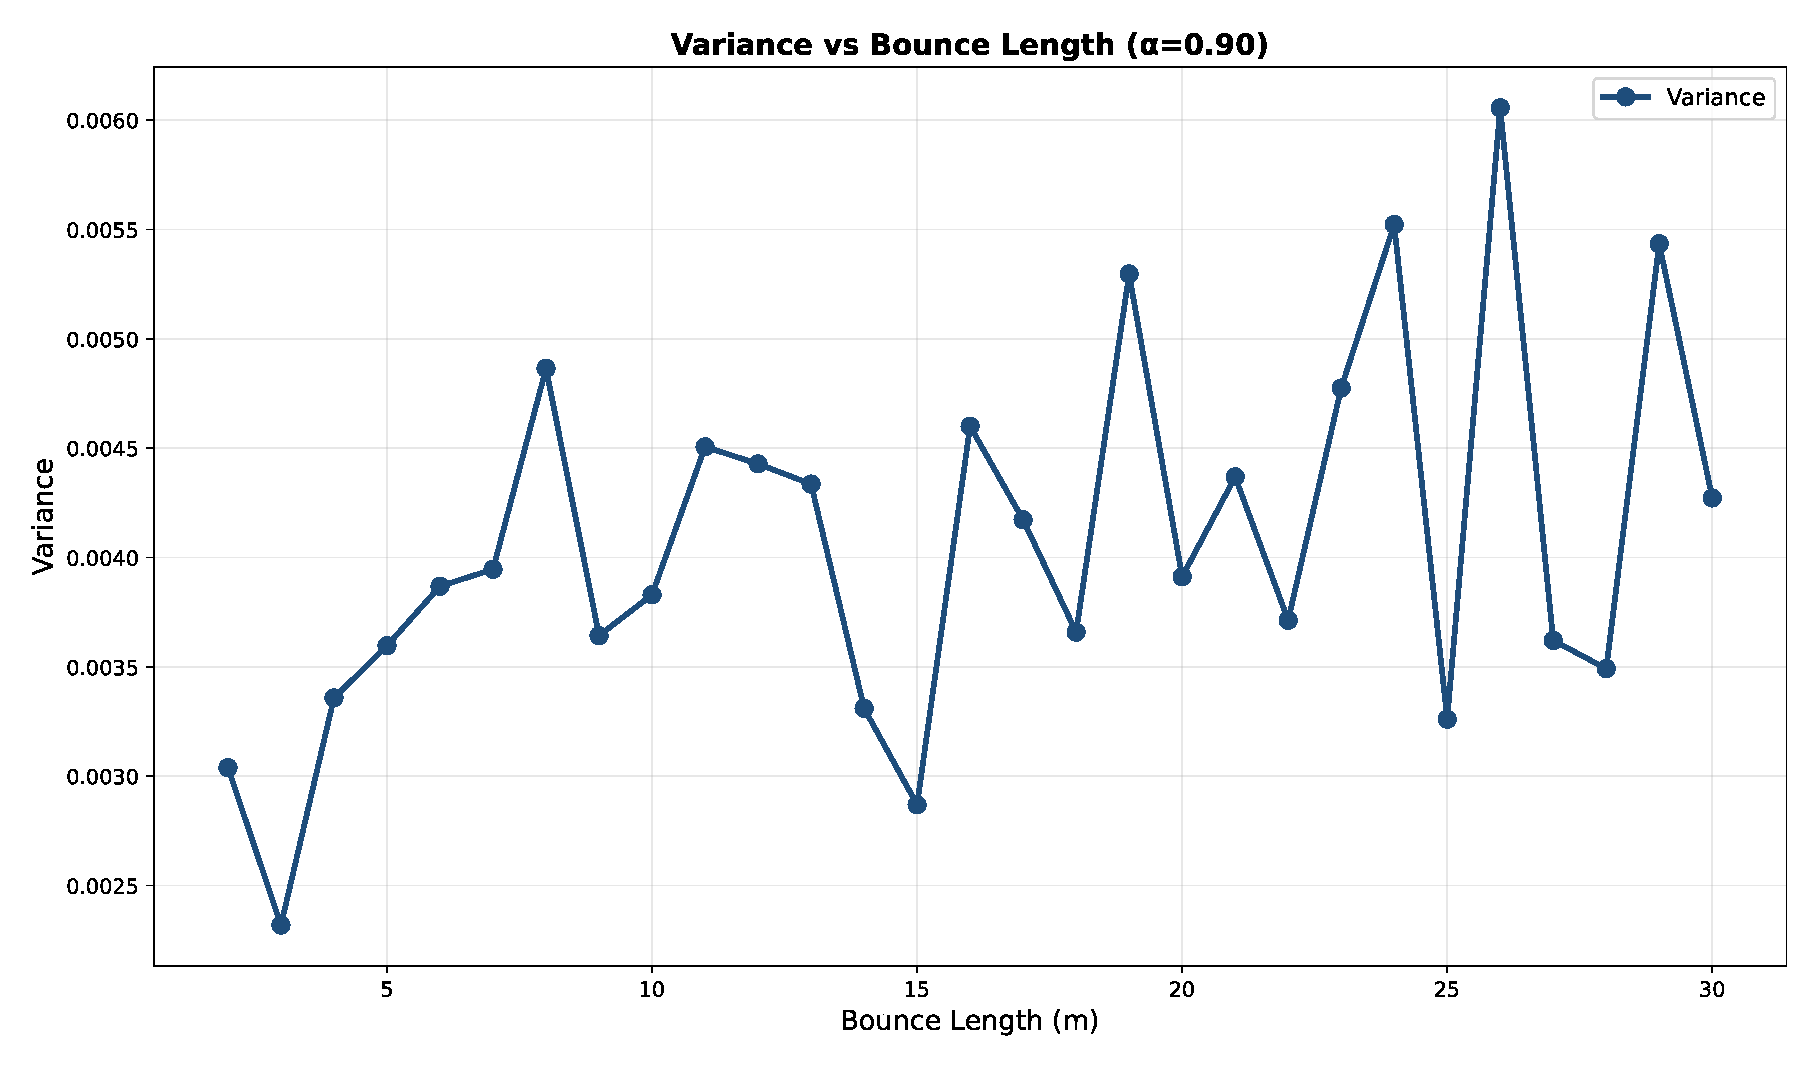
\includegraphics[width=0.8\textwidth]{figure/variance_alpha0.90_m2-30.eps}
    \caption{Variance vs Bounce Number ($\alpha=0.90$, m2-30)}
    \label{fig:variance_alpha0.90}
\end{figure}

\begin{figure}[htbp]
    \centering
    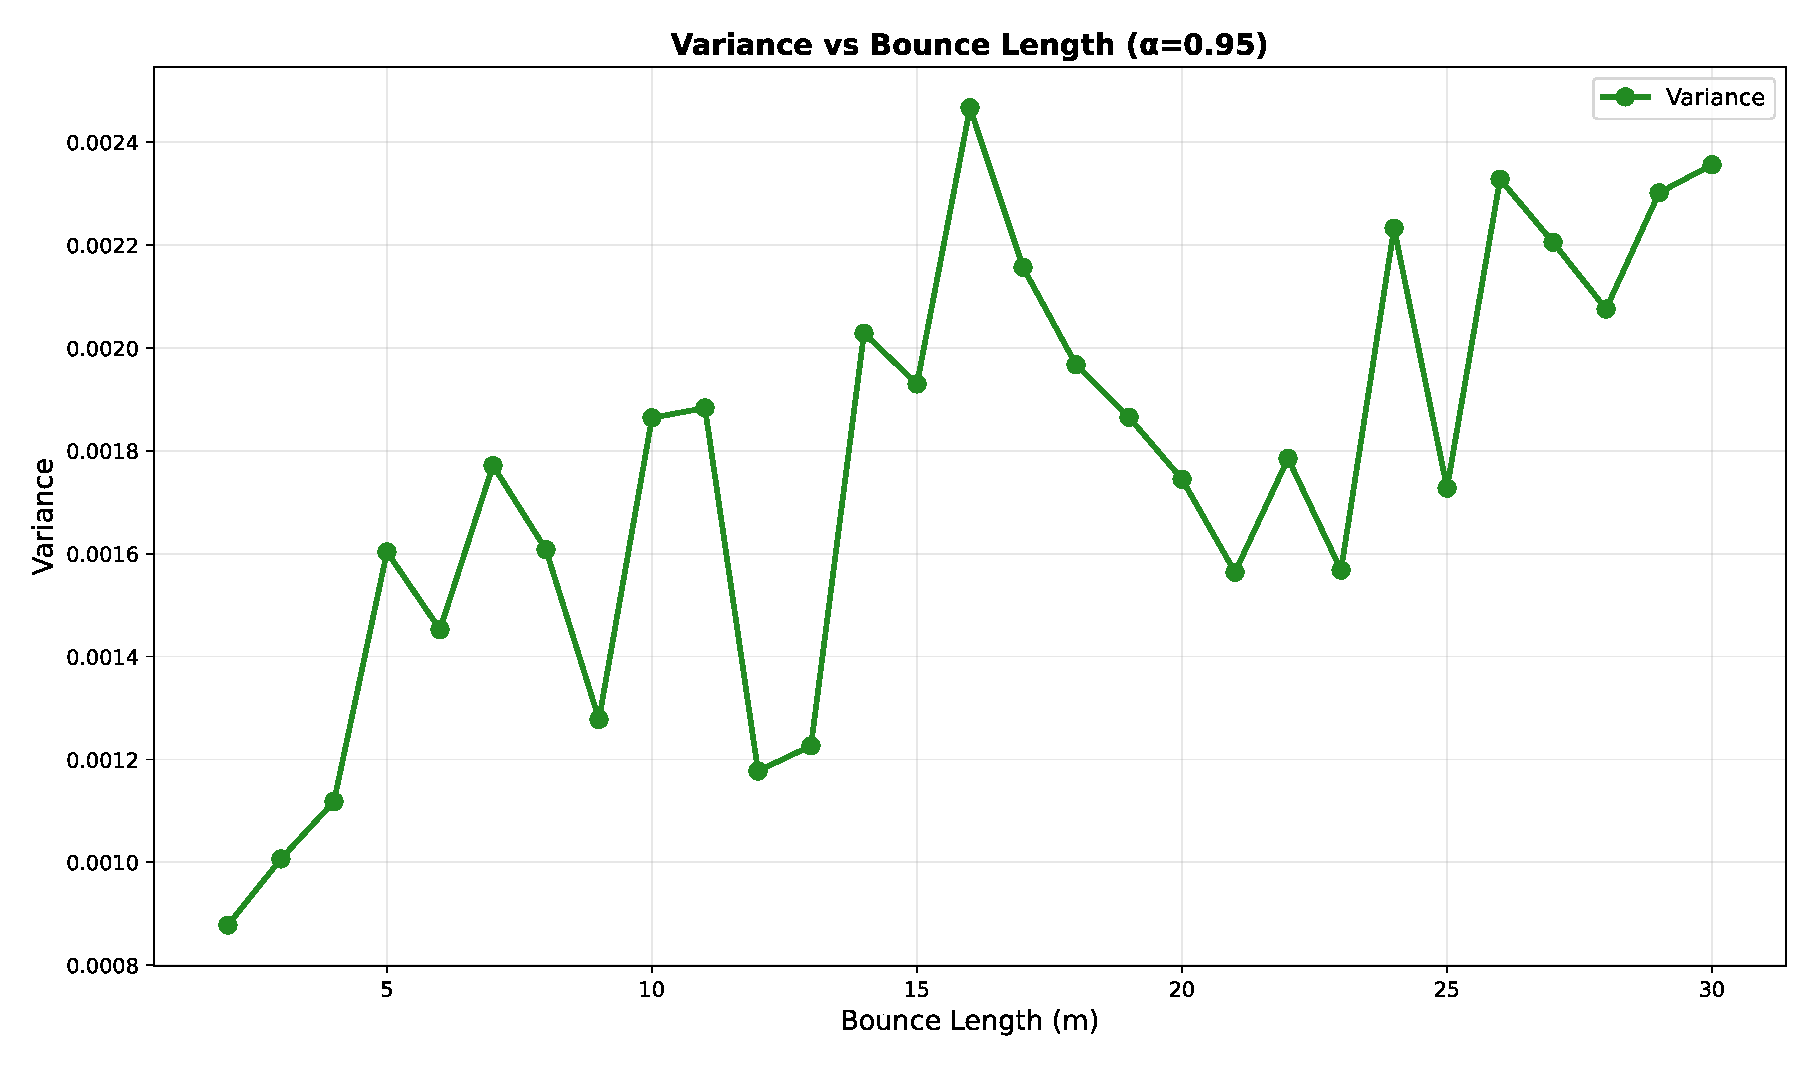
\includegraphics[width=0.8\textwidth]{figure/variance_alpha0.95_m2-30.eps}
    \caption{Variance vs Bounce Number ($\alpha=0.95$, m2-30)}
    \label{fig:variance_alpha0.95}
\end{figure}

\begin{figure}[htbp]
    \centering
    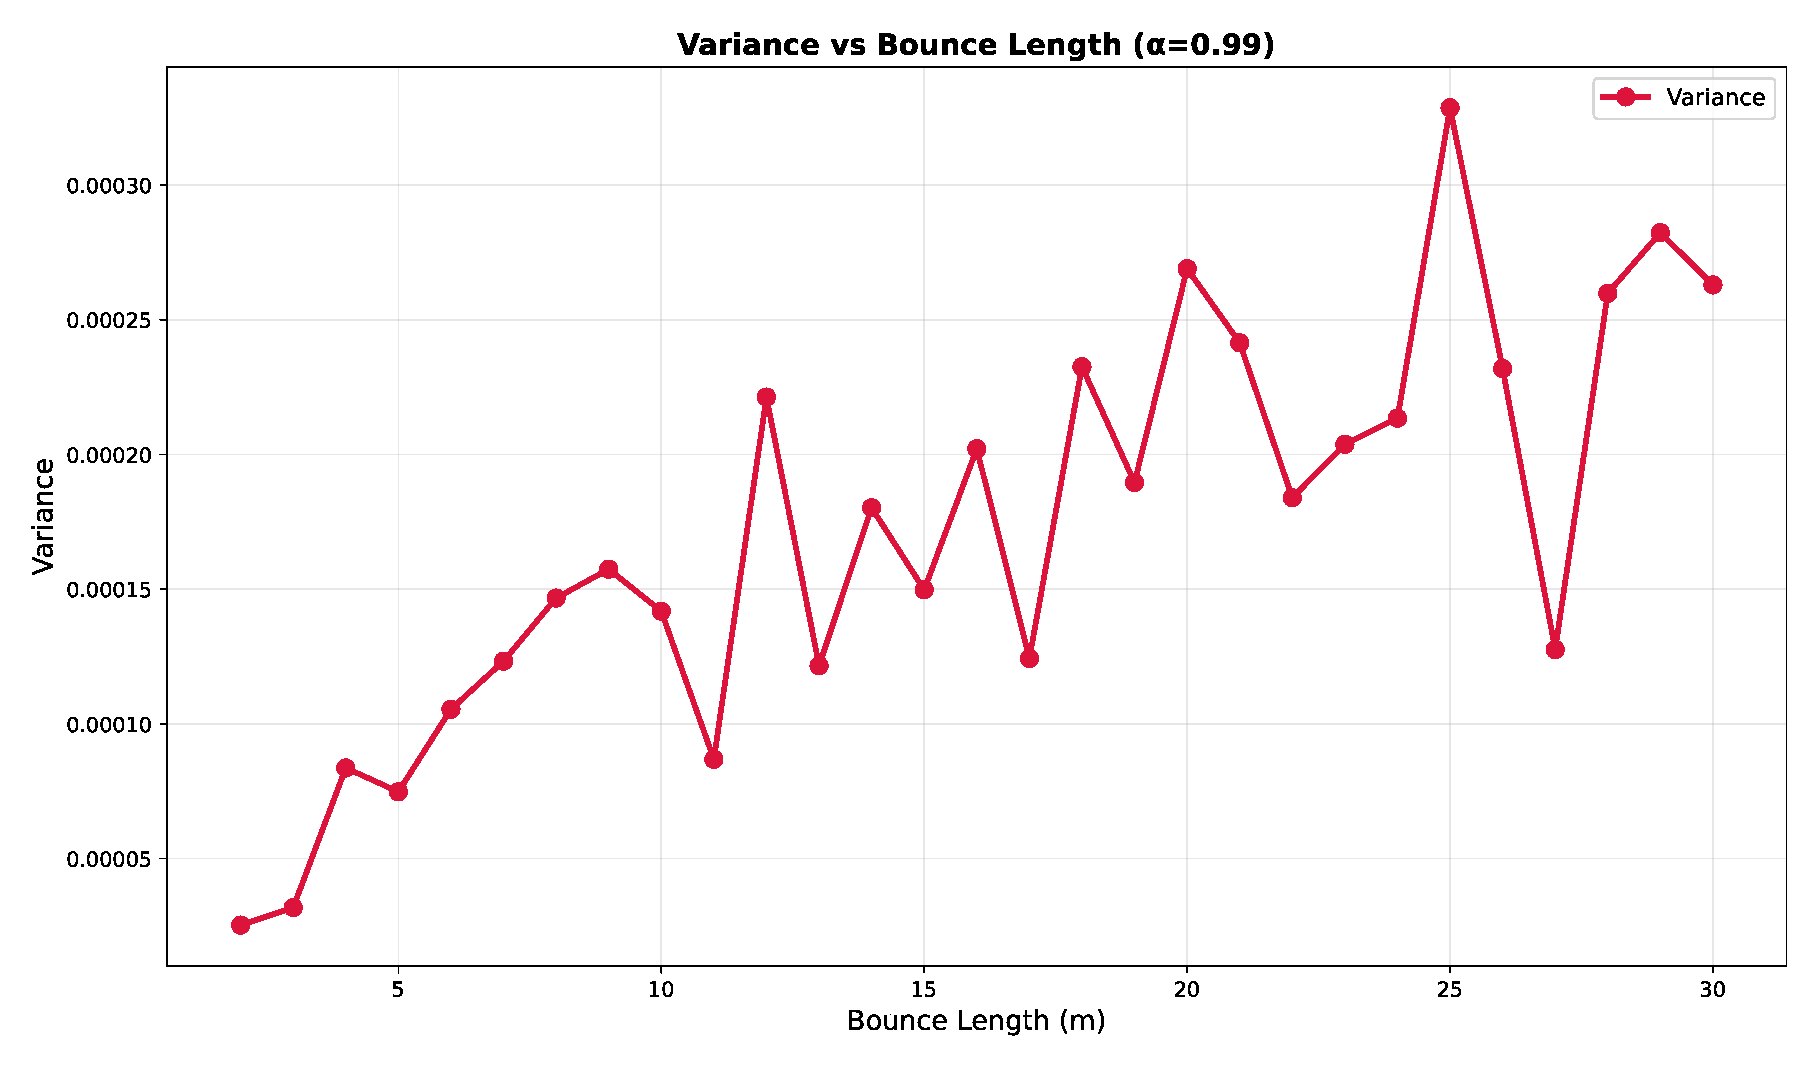
\includegraphics[width=0.8\textwidth]{figure/variance_alpha0.99_m2-30.eps}
    \caption{Variance vs Bounce Number ($\alpha=0.99$, m2-30)}
    \label{fig:variance_alpha0.99}
\end{figure}

図\ref{fig:variance_alpha0.90}～図\ref{fig:variance_alpha0.99}は、各データ点 $\bar{b}_m$ のばらつきがどのように変化するかを可視化した図である。

バウンス数 $m$ は2から30の範囲で変化させた。各バウンス数につき、40通りのランダムなゲートシーケンスを実行した。

実験設定として、輝度状態（bright state）の占有率を表わす $alpha$ の値を3段階に設定した。NBでは $alpha=0.95$ が選択されているが、著者らも述べている通り、これはモデルの元となった実際の実験値（Humphreys et al.）とはわずかに異なる値である。そのため、本研究ではNBの再現となる $alpha=0.95$ に加え、当時の実験的な実測値により近い $alpha=0.90$、および量子誤り訂正などを見据えた将来的な高品質リンクを想定した $alpha=0.99$ の3つの輝度状態（bright state）の占有率においてシミュレーションを行なった。


分散はバウンス数 $m$ と共に増大する傾向にあるが、その振る舞いは単調ではない。特に $\alpha=0.90$ のような低品質な領域では、信号の減衰に伴う分散のベースラインの上昇に加え、有限サンプリングに起因する大きな変動が観測される。特に注目すべきは、バウンス数 $m$ が小さい範囲（初期領域）における分散の振る舞いである。しかし、図\ref{fig:variance_alpha0.90}～図\ref{fig:variance_alpha0.99}のいずれの条件下においても、初期の $m$ （概ね $m \leq 10$）の範囲では、分散は $m$ の増加に対して一貫した増大傾向を示している。初期段階では信号強度が十分に高いため、統計的なゆらぎ（サンプリングごとのばらつき）よりも、脱分極に伴う体系的な不確定性の増大が支配的となっていることを示している。

\begin{table}[htbp]
    \centering
    \caption{Fidelity Estimation Results ($\alpha=0.90$, N=40)}
    \label{tab:fidelity_alpha0.90}
    \begin{tabular}{c|cc}
    \hline
    $m$ range & OLS & WLS \\
    \hline
    m2-10 & $0.8215 \pm 0.0091$ & $0.8206 \pm 0.0070$ \\
    m2-20 & $0.8179 \pm 0.0076$ & $0.8185 \pm 0.0056$ \\
    m2-30 & $0.8191 \pm 0.0090$ & $0.8191 \pm 0.0055$ \\
    \hline
    \end{tabular}
\end{table}

\begin{table}[htbp]
    \centering
    \caption{Fidelity Estimation Results ($\alpha=0.95$, N=40)}
    \label{tab:fidelity_alpha0.95}
    \begin{tabular}{c|cc}
    \hline
    $m$ range & OLS & WLS \\
    \hline
    m2-10 & $0.9080 \pm 0.0063$ & $0.9073 \pm 0.0025$ \\
    m2-20 & $0.9029 \pm 0.0033$ & $0.9029 \pm 0.0015$ \\
    m2-30 & $0.9006 \pm 0.0029$ & $0.9010 \pm 0.0013$ \\
    \hline
    \end{tabular}
\end{table}

\begin{table}[htbp]
    \centering
    \caption{Fidelity Estimation Results ($\alpha=0.99$, N=40)}
    \label{tab:fidelity_alpha0.99}
    \begin{tabular}{c|cc}
    \hline
    $m$ range & OLS & WLS \\
    \hline
    m2-10 & $0.9752 \pm 0.0041$ & $0.9765 \pm 0.0004$ \\
    m2-20 & $0.9764 \pm 0.0018$ & $0.9763 \pm 0.0002$ \\
    m2-30 & $0.9761 \pm 0.0009$ & $0.9762 \pm 0.0001$ \\
    \hline
    \end{tabular}
\end{table}

表\ref{tab:fidelity_alpha0.90}～表\ref{tab:fidelity_alpha0.99}は、各リンク品質 $\alpha \in \{0.90, 0.95, 0.99\}$ において、バウンス数の測定範囲（$m$ range）を 2-10、2-20、2-30 と変化させ各 $m$ に対して40回の測定を行なった時点での、OLSおよびWLSによる忠実度推定値とその標準誤差（Standard Error）をまとめたものである。標準誤差の大きさについて比較すると、全ての $\alpha$ および全ての測定範囲において、WLSによる推定値の標準誤差はOLSのそれよりも小さな値を示した。

しかし、表\ref{tab:fidelity_alpha0.95}（$\alpha=0.95$）の結果において、測定範囲を $m=2\text{-}10$ に制限した際のWLS推定値（$0.9073$）は、全範囲 $m=2\text{-}30$ を用いた際の推定値（$0.9010$）と比較して、標準誤差の範囲を超えた有意な乖離を示している。通常のOLSを用いた場合、短尺測定では標準誤差が大きくなるため（$\pm 0.0063$）、推定値に含まれる系統的なバイアスは誤差範囲内に埋没し、統計的には矛盾しない結果として解釈されうる。しかし、WLSを導入した場合、その標準誤差は劇的に縮小される（$\pm 0.0025$）。この極めて高い精度ゆえに、OLSでは許容されていたわずかな系統誤差が、統計的に有意な誤りとして露呈する結果となった。この現象は、WLSが有限サンプリングに起因する分散の局所的なバラつきに対して過剰に適合し、特定のデータ点に偏った重み付けを行ってしまったことに起因すると考えられる。

\begin{figure}[htbp]
    \centering
    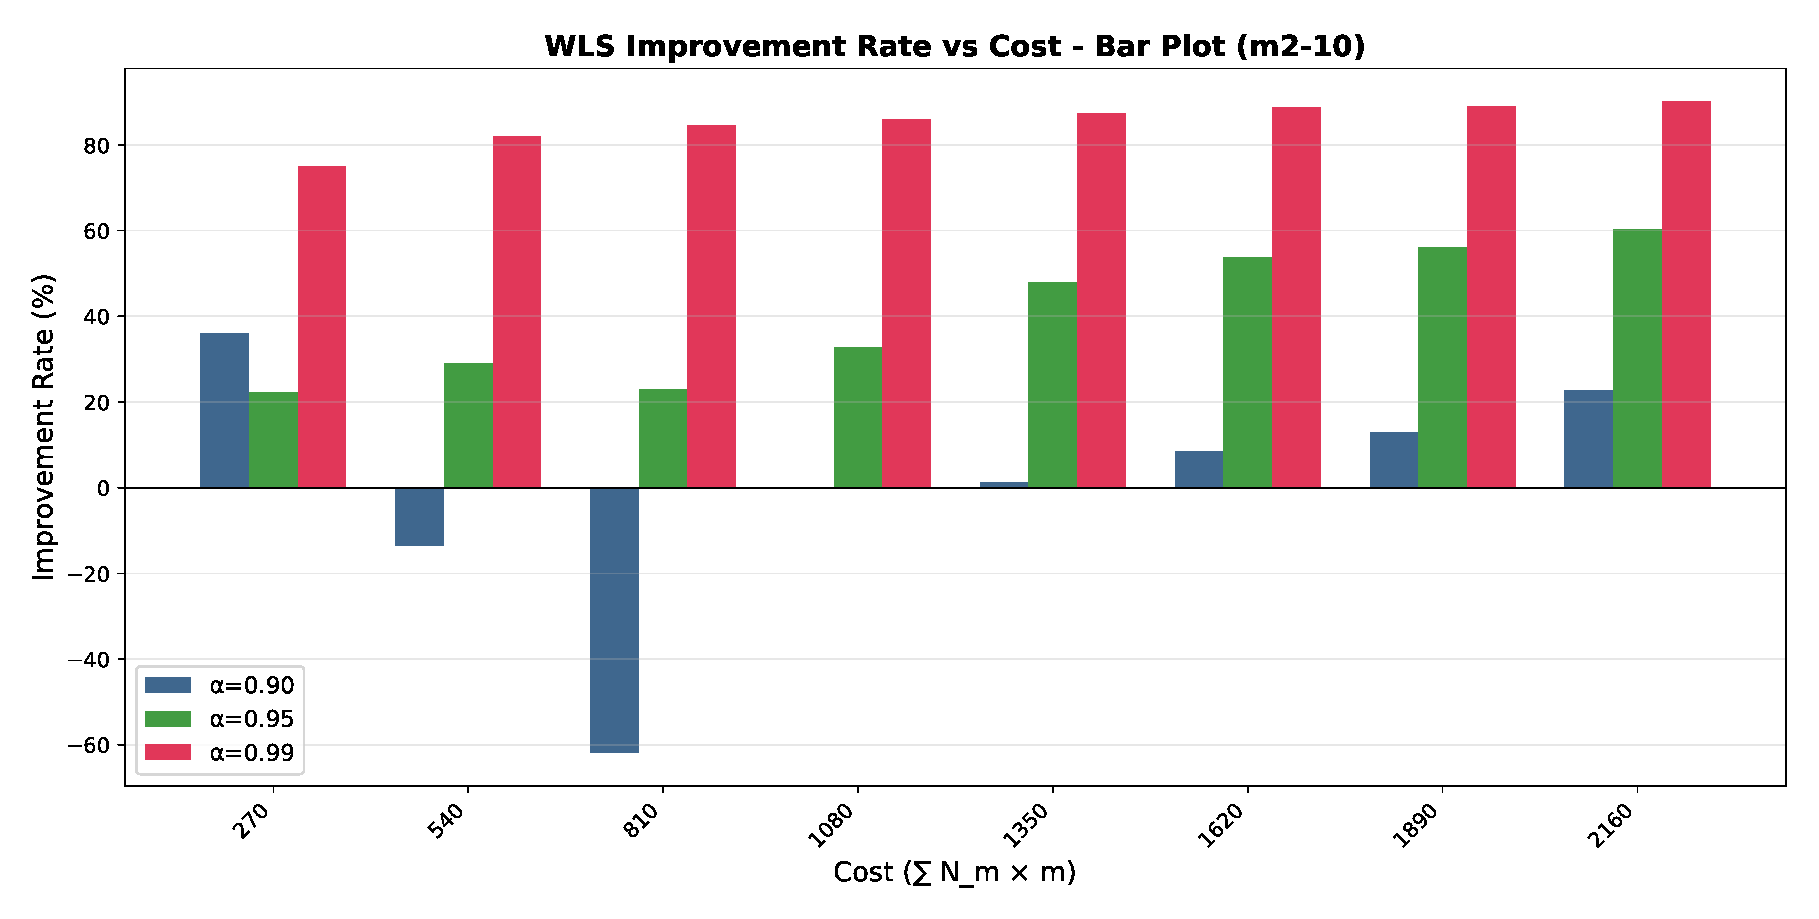
\includegraphics[width=0.8\textwidth]{figure/improvement_rate_bar_m2-10.eps}
    \caption{Improvement Rate of Standard Error (m2-10)}
    \label{fig:improvement_rate_m2-10}
\end{figure}

\begin{figure}[htbp]
    \centering
    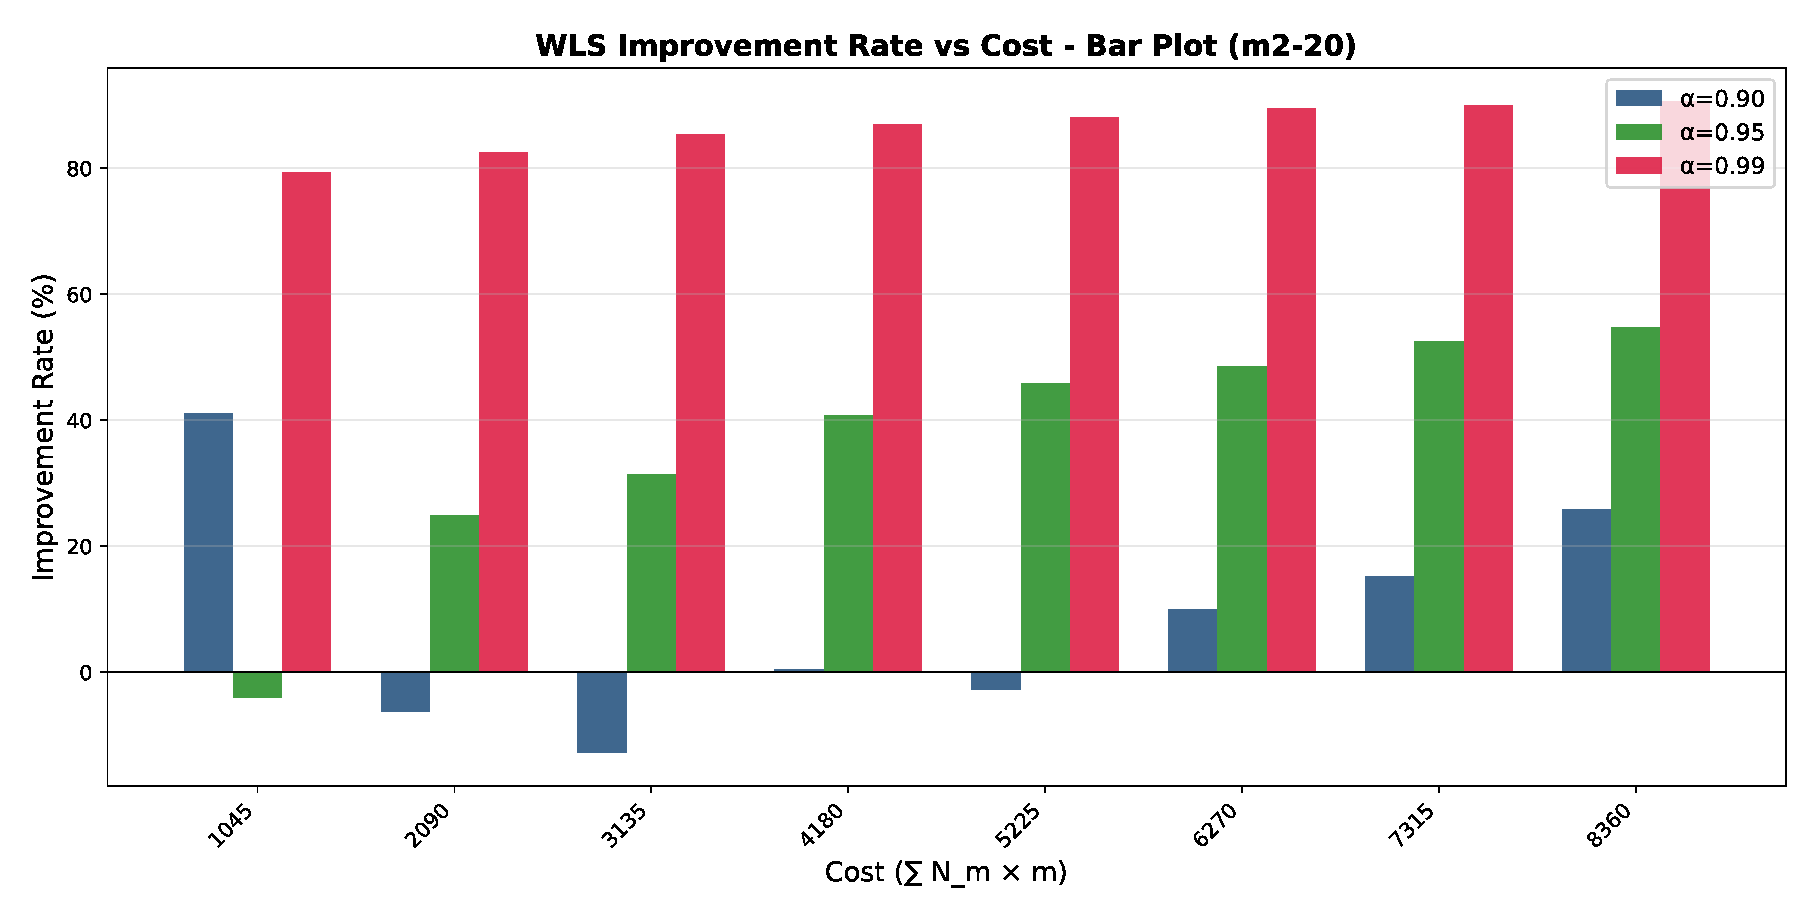
\includegraphics[width=0.8\textwidth]{figure/improvement_rate_bar_m2-20.eps}
    \caption{Improvement Rate of Standard Error (m2-20)}
    \label{fig:improvement_rate_m2-20}
\end{figure}

\begin{figure}[htbp]
    \centering
    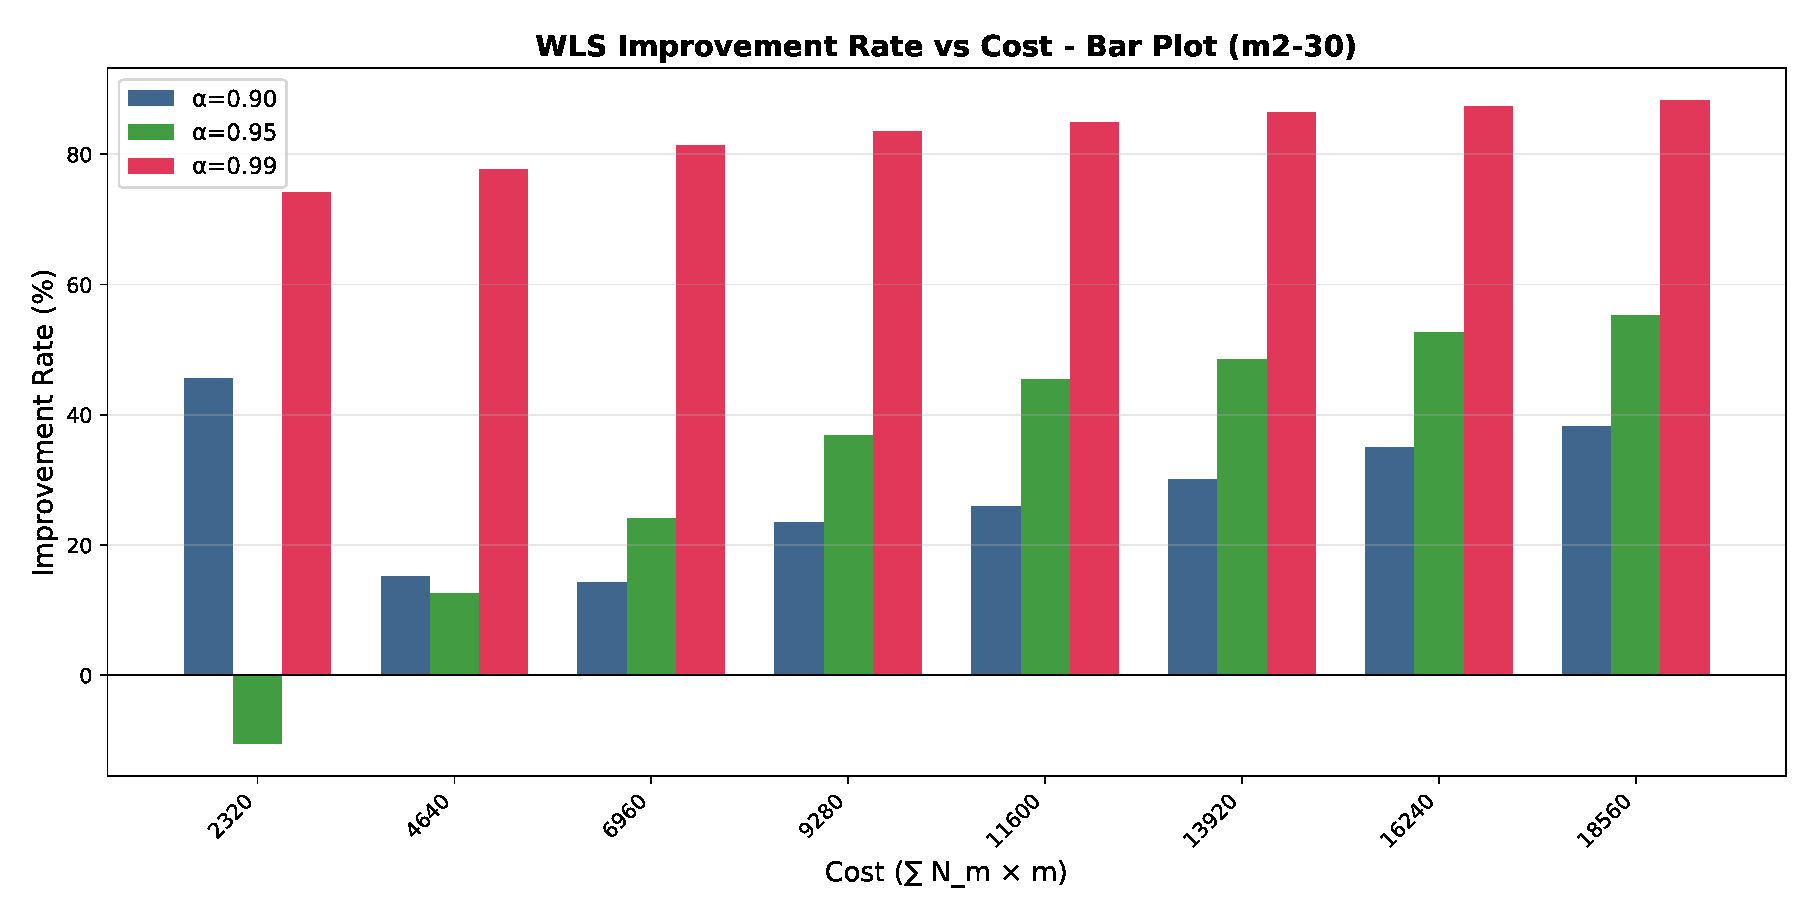
\includegraphics[width=0.8\textwidth]{figure/improvement_rate_bar_m2-30.eps}
    \caption{Improvement Rate of Standard Error (m2-30)}
    \label{fig:improvement_rate_m2-30}
\end{figure}

図\ref{fig:improvement_rate_m2-10}～図\ref{fig:improvement_rate_m2-30} は、各条件におけるWLSの導入効果を定量化するため、OLSに対する標準誤差の改善率を、実験コストの関数としてプロットしたものである。ネットワークベンチマークでは、長距離にわたって量子ビットを送信するコストがサンプルのコストにおける支配的な要因となるため、$m$ バウンスを含むシーケンスのサンプリングは、1バウンスのみを含むシーケンスのサンプリングよりもおよそ $m$ 倍高価になる。ゆえに、$\sum_{m \in \mathbb{M}} N_m \cdot m$とコストを定義した。

まず、高品質なリンク（$\alpha=0.99$、赤色のバー）に着目すると、コストの大小や測定範囲（$m$-range）に関わらず、一貫して80\%前後の極めて高い改善率を示している。これは、信号の減衰が緩やかで分散の推定が安定しているため、WLSが理想的に機能していることを示している。

一方で、リンク品質が低い（$\alpha=0.90$）ケースでは、図\ref{fig:improvement_rate_m2-10}（$m=2\text{-}10$）の低コスト領域（左側のバー群）に見られるように、改善率（$\text{改善率 (\%)} = (\text{OLSの絶対不確実性} - \text{WLSの絶対不確実性}) / \text{OLSの絶対不確実性} \times 100$）が負の値を示している箇所が存在する。この現象の原因は、重み $w_m$ 自体の推定誤差にある。WLSの重みは標本分散の逆数 $(1/\sigma_m^2)$ として算出されるが、サンプル数 $N_m$ が少ない場合（低コスト時）、この標本分散自体が大きな統計的ゆらぎを持つ。特にノイズの大きい低品質リンクでは、誤った重みが算出されやすく、その結果としてフィッティングが不安定化したと考えられる。

しかし、コストが増加しサンプル数 $N_m$ が十分に確保されるにつれて、$\alpha=0.90$ および $\alpha=0.95$ の改善率は着実に上昇し、正の値へと転じている。これは、サンプル数の増加に伴い分散の推定精度が向上し、適切な重み付けが可能になった結果である。


%------------------------------
\newpage
\section{Conclusion}
\label{sec:conclusion}
本研究では、量子ネットワークリンクの品質推定における Network Benchmarking (NB) プロトコルのデータ処理手法について検討を行った。特に、フィッティング手法として従来の最小二乗法 (OLS) と、分散の不均一性を考慮した最小二乗法 (WLS) の性能比較を、NetSquid シミュレーションにより実施した。シミュレーションの結果、WLS は OLS と比較して、特にリンク忠実度が高い領域（$\alpha=0.99$）において推定値の標準誤差を有意に低減できることが確認された。これは、バウンス回数 $m$ の増加に伴う分散の変動（不均一分散）に対し、WLS が分散の逆数を重みとして用いることで、より適切なフィッティングを実現したためであると考えられる。

本研究によりWLSの有効性が示された一方で、実用化に向けて解決すべき課題も浮き彫りとなった。特に低忠実度領域（$\alpha=0.90$）においては、分散推定の不安定さにより改善幅が限定的となる傾向が見られた。また、特定の条件下（$\alpha=0.95$）では、WLSが有限サンプリングに伴う分散の局所的なばらつきに過剰適合し、OLSでは統計的に許容される微小なバイアスを有意な乖離として顕在化させる現象も確認された。これらの課題に対処するためには、ノイズレベルに応じた適切な手法の選択や、よりロバストな分散推定法の適用といった基礎的な改善が求められる。

本手法の今後の展望としては、各バウンス回数 $m$ に対して異なる測定回数（$N_m$）を割り当てた際の分散の変化に対する重み付けの検討が挙げられる。本研究では $m$ の増加に起因する分散の変動に対して WLS の重み付けが有効であることを示したが、今後は $N_m$ を不均一に配分することで生じる分散の差異に対しても、WLS による重み付けを適用し、その挙動や有効性を検証する必要がある。これにより、総測定コストと推定精度のトレードオフを考慮した、より柔軟で効率的な測定設計への指針が得られる可能性がある。



\newpage

\appendix

\section*{Acknowledgments}
\addcontentsline{toc}{section}{Acknowledgments}


I would like to express my sincere gratitude to all those who supported and assisted me in completing this research.

First and foremost, I wish to express my deepest appreciation to Prof. Hiroyuki Ohsaki for his invaluable guidance and continuous advice throughout this work. I am also profoundly grateful to Prof. Nagisa Ishiura and Prof. Akihiro Inokuchi for their rigorous guidance and insightful comments during the interim review; their feedback was instrumental in deepening the scope of this research.

I would like to thank Mr. Shota Inoue and Mr. Yuto Kakihara, and all the members of the Ohsaki Laboratory for their helpful discussions and daily support.



\newpage

%% \renewcommand{\em}{\it}
%% \bibliographystyle{ieeetr}
\renewcommand{\em}{\it}
\bibliographystyle{ieeetr}
\addcontentsline{toc}{section}{\refname}
\bibliography{./../bib/references}


\end{document}
